\documentclass[serif, aspectratio=169]{beamer}
%\documentclass[serif]{beamer}  % for 4:3 ratio

\usepackage[T1]{fontenc} 
\usepackage[utf8]{inputenc}
\usepackage{fourier} % see "http://faq.ktug.org/wiki/uploads/MathFonts.pdf" for other options
\usepackage{hyperref}
\usepackage{latexsym,amsmath,xcolor,multicol,booktabs,calligra}
\usepackage{graphicx,pstricks,listings,stackengine}
\usepackage{lipsum}
\usepackage{../HKUSTstyle}

%imports customs%
\usepackage{caption}    % for subfigures
\usepackage{subcaption} % for subfigures
\usepackage{ragged2e}
\usepackage{booktabs,makecell}
\usepackage{colortbl}
\usepackage{multirow}
\usepackage{cite}
\usepackage{tcolorbox}
\usepackage[sort,authoryear]{natbib}

\author{Julien Bezançon}

\title{Python Programmation}
\subtitle{CM 1~: Welcome and Introduction}

\institute{julien.bezancon@univ-lorraine.fr / \url{https://julienbez.github.io}}

\date{}

% defs
\def\cmd#1{\texttt{\color{red}\footnotesize $\backslash$#1}}
\def\env#1{\texttt{\color{blue}\footnotesize #1}}

% set colors
\definecolor{hkustyellow}{RGB}{167, 131, 55}
\definecolor{hkustblue}{RGB}{0, 56, 116}
\definecolor{hkustred}{RGB}{209, 51, 59}

% easy colors
\newcommand{\tred}[1]{\textcolor{red!50}{#1}}
\newcommand{\tgreen}[1]{\textcolor{green}{#1}}
\newcommand{\tyellow}[1]{\textcolor{yellow}{#1}}
\newcommand{\tpurple}[1]{\textcolor{purple!50}{#1}}

% CLI environment
\newenvironment{CLI} % Command Line Interface
    {
    \noindent
    \ttfamily 
    \footnotesize
    \begin{tcolorbox}[colback=gray!150,colframe=black]
    \color{white}
    \begin{tabular}{p{4.5cm}p{7.5cm}}
    }
    { 
    \end{tabular}
    \end{tcolorbox}
    }

% Exercice environment
\newenvironment{exoframe}
    {
    \setbeamercolor{background canvas}{bg=hkustblue}
    \renewcommand\thefootnote{\textcolor{white}{\arabic{footnote}}}
    \color{white}
    \setbeamercolor{structure}{fg=white}
    \begin{frame}
    }
    {
    \end{frame}
    }

\lstset{
    basicstyle=\ttfamily\small,
    keywordstyle=\bfseries\color{deepblue},
    emphstyle=\ttfamily\color{deepred},    % Custom highlighting style
    stringstyle=\color{deepgreen},
    numbers=left,
    numberstyle=\small\color{halfgray},
    rulesepcolor=\color{red!20!green!20!blue!20},
    frame=shadowbox,
}

\begin{document} %  --- --- --- --- --- --- --- --- --- --- --- --- 

\begin{frame}[noframenumbering,plain]
    \titlepage
    \vspace*{-0.6cm}
    \begin{figure}[htpb]
        \begin{center}
            \hspace{0.3cm}
            
\includegraphics[width=0.7\columnwidth]{../../../IMAGES/loria_idmc.png}
        \end{center}
    \end{figure}
\end{frame}

% \begin{frame}    
%     \tableofcontents[sectionstyle=show,
%     subsectionstyle=show/shaded/hide,
%     subsubsectionstyle=show/shaded/hide]
% \end{frame}

\section{Before we start...}

\begin{frame}{About me} %Julien Bezançon

    % \begin{figure}
    %     
\includegraphics[width=0.5\columnwidth]{../../../FIGURES/photos/profile_thug.jpeg}
    % \end{figure}

    \begin{minipage}{0.45\columnwidth}
        \begin{figure}
            
\includegraphics[width=0.7\columnwidth]{../../../FIGURES/photos/profile_thug.jpeg}
        \end{figure}
    \end{minipage}
    \begin{minipage}{0.45\columnwidth}
        \begin{block}{You will see me in...}
            \vspace{5pt}
            \begin{itemize}
                \item Data Storage and Retrieval \hfill M1
                \item Prompt Engineering \hfill M2
                \item Software Projects \hfill M2
                \item Written Corpora \hfill M2
                \item Lexicology \hfill M2
            \end{itemize}
        \end{block}
    \end{minipage}
\end{frame}

\begin{frame}{About this course} %-- 8 weeks, 4 hours a week
    \begin{block}{8 lectures (CM), each one followed by a practical session (TD)}
        \begin{itemize}
            \item General Introduction
            \item Data Structure
            \item Functions
            \item Object-Oriented Python
            \item Functional Programming
        \end{itemize}
    \end{block}
    \pause
    \begin{block}{Evaluation mode}
        \begin{itemize}
            \item Practical sessions (50~\%) 
            \item Final exam (50~\%)
        \end{itemize}
    \end{block}
    \pause
    \hfill \textbf{Final exam~: 30/11/2026}
\end{frame}

\begin{frame}{About the practical sessions}
    \begin{block}{For each practical session...}
        \begin{itemize}
            \item Download the notebook on Arche
            \item Complete it and put it back on Arche
        \end{itemize}
    \end{block}
    \begin{block}{}
        \begin{itemize}
            \item 3 random practical sessions will be graded
            \item the worst grade \textit{can} be removed
        \end{itemize}
    \end{block}
\end{frame}

\begin{frame}{References for this course}
    \begin{block}{}
        \begin{itemize}
            \item Tom Bourgeade (tom.bourgeade@loria.fr)
            \item Sam Redmon (sredmond@stanford.edu)
            % \item Karën Fort (karen.fort@univ-lorraine.fr)
            \item Python documentation\footnote{\url{https://docs.python.org/3/}}
        \end{itemize}
    \end{block}
\end{frame}

\section{Introduction}

\begin{frame}{What is Python ?}
    \begin{block}{Python is a programming language}
        \begin{itemize}
            \item Who ? Guido van Rossum, a.k.a the \textit{Benevolent Dictator for Life}
            \item Why ? Because he wanted a hobby during christmas
            \item The name ? A reference to \textit{Monty Python's Flying Circus}
        \end{itemize}
    \end{block}
    \pause
    \begin{block}{Python is an ongoing project}
        \begin{itemize}
            \item Python 1~: 1994
            \item Python 2~: 2000
            \item Python 3~: 2008
            \vspace{5pt}
            \item As of today~: Python 3.14.7
        \end{itemize}
    \end{block}
    \pause
    \hfill \textbf{Why should I use Python ?}
\end{frame}

\begin{frame}{First reason~: It's easy}
    \begin{block}{The "Hello World" script}
        \begin{figure}
            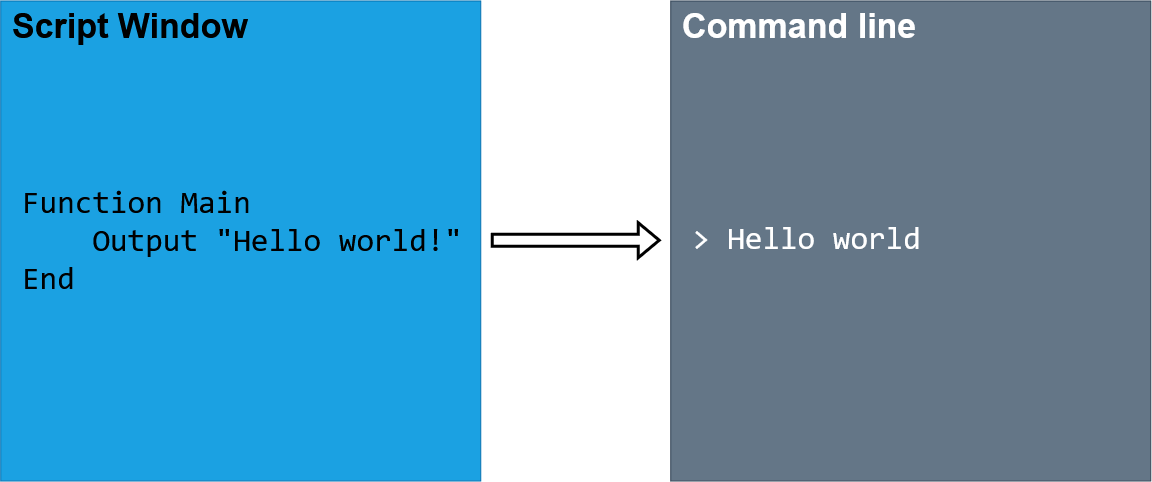
\includegraphics[width=0.9\columnwidth]{../../../FIGURES/python/hello_world_pseudocode.png}
            %\caption{}
        \end{figure}
    \end{block}
\end{frame}

\begin{frame}{First reason~: It's easy}
    \begin{block}{"Hello World" in Java}
        \vspace{2pt}
        \begin{CLI}
            \textcolor{blue!50}{public class} \textcolor{green!50}{HelloWorld} \{ & \\
            \multicolumn{2}{l}{~~\textcolor{blue!50}{public static} \textcolor{green!50}{void} \textcolor{purple!50}{main(String[] args)} \{ } \\
            \multicolumn{2}{l}{~~~~ System.out.\textcolor{purple!50}{println}\textcolor{blue!50}{("Hello World")};} \\
            ~~ \} & \\
            \} & \\
        \end{CLI}
    \end{block}
\end{frame}

\begin{frame}{First reason~: It's easy}
    \begin{block}{"Hello World" in C++}
        \vspace{2pt}
        \begin{CLI}
            \textcolor{purple!50}{\#include} \textcolor{blue!50}{<iostream>} & \\
            \textcolor{purple!50}{using} \textcolor{blue!50}{namespace} \textcolor{green!50}{std}; & \\
            & \\
            \textcolor{red!50}{int} \textcolor{purple!50}{main()} \{ & \\
            \multicolumn{2}{l}{~~cout $<$$<$ \textcolor{blue!50}{"Hello World"};} \\
            \multicolumn{2}{l}{~~\textcolor{purple!50}{return} 0;} \\
            \} & \\
        \end{CLI}
    \end{block}
\end{frame}

\begin{frame}{First reason~: It's easy}
    \begin{block}{"Hello World" in Python}
        \vspace{2pt}
        \begin{CLI}
            \textcolor{purple!50}{print}(\textcolor{blue!50}{"Hello World"}) & \\
        \end{CLI}
    \end{block}
\end{frame}

\begin{frame}{Second reason~: Python  is very interactive}
    \begin{block}{Python can even be used in the command line !}
        \vspace{2pt}
        \begin{CLI}
            \multicolumn{2}{l}{C:/Users/julien/documents/github > python} \\
            & \\
            \multicolumn{2}{l}{Python 3.13.14 (tags/v3.13.14:fd17997, Jun 10 2026, 13:03:48) on win32} \\
            \multicolumn{2}{l}{Type "help", "copyright", "credits" or "license" for more information.} \\
            & \\
            \multicolumn{2}{l}{$>$$>$$>$ \only<2->{print("Hello World")}} \\
            \only<2->{Hello World} & \\
            & \\
            & \\
        \end{CLI}
    \end{block}
\end{frame}

\begin{frame}{Second reason~: Python is very interactive}
    \begin{block}{Why does it matter ?}
        \begin{itemize}
            \item Immediate gratification
            \item Lots of freely available resources to learn Python
            \item Shortens code-test-debug cycle to seconds
        \end{itemize}
    \end{block}
    \pause
    \begin{block}{Python is also...}
        \begin{itemize}
            \item Easy to install (Linux, Windows, IOS,etc)
            \item Modular (you can import libraries)
            \item + you can contribute to Python !
        \end{itemize}
    \end{block}
\end{frame}

\begin{frame}{Third reason~: Python is widely used}
    \begin{block}{Who uses Python ?}
        \begin{itemize}
            \item Researchers from various fields (NLP, astronomy, biology, social sciences, etc)
            \pause
            \item Manufacturers and companies of all size
        \end{itemize}
    \end{block}
    \pause
    \begin{block}{}
        \begin{figure}
            
\includegraphics[width=0.55\columnwidth]{../../../FIGURES/python/companies.png}
            \caption{Some examples of companies using Python}
        \end{figure}
    \end{block}
\end{frame}

\begin{frame}{Third reason~: Python is widely used}
    \begin{block}{More specifically, Python is used for...}
        \begin{itemize}
            \item Data science, Statistical analysis
            \item Software development
            \item Cybersecurity
            \item Financial technologies
            \item Artificial Intelligence
            \item Web development
            \item Machine Learning systems
        \end{itemize}
    \end{block}
    \hfill \textbf{And the list goes on...}
\end{frame}

\begin{frame}{A Quick summary}
    \begin{block}{Python is...}
        \begin{itemize}
            \item Popular (million of users worldwide)
            \item Practical (easy to install, easy to use)
            \item Still evolving\footnote{\url{https://devguide.python.org/versions/}}
        \end{itemize}
    \end{block}
    \pause
    \begin{block}{During this course, you will...}
        \begin{itemize}
            \item Develop skills with Python fundamentals
            \item Learn to recognize "bad" Python and to write "good" Python
            \item Frequently practice python, both during lectures and practical sessions
        \end{itemize}
        
    \end{block}
    % \begin{block}{What are the goals of this course ?}
    %     \begin{itemize}
    %         \item Develop skills with Python fundamentals
    %         \item Learn to recognize and write "good" Python
    %         \item Gain experience with practical Python tasks
    %         \item Understand Python's strengths (and weaknesses)
    %     \end{itemize}
    % \end{block}
\end{frame}


\begin{exoframe}
    \begin{center}
            \Large
            Install Python: \url{https://www.python.org/downloads/}
    \end{center}
    \vspace{10pt}
    \begin{center}
        \Large
        Do you have a Python editor on your computer ? \\
        If not, then install one (e.g: Jupyter Notebook\footnote{\color{white} \url{https://jupyter.org/install}})
    \end{center}
\end{exoframe}

\section{The Basics of Python}

\begin{frame}{Variables}
    \begin{CLI}
        x = 42 & \\
        sentence = "Hello" & \\
        \pause
        & \\
        x * 2 & \\
        sentence + "World" & \\
    \end{CLI}
    \pause
    \begin{block}{Questions}
        \begin{itemize}
            \item What is the difference between these two variables ? \only<4->{$\Rightarrow$ their type}
            \item Is there a way to show this difference in Python ? \only<5->{$\Rightarrow$ type()}
            \item What would be the result of these operations ? \only<6->{$\Rightarrow$ 84 and "Hello World"}
        \end{itemize}
    \end{block}
\end{frame}

\begin{frame}{Types}
    \begin{CLI}
        x = 42 & \\ 
        sentence = "Hello" & \\
        & \\
        type(x) & \\
        type(sentence) & \\
    \end{CLI}
    \pause
    \begin{block}{Questions}
        \begin{itemize}
            \item What is the type of \textbf{x} ? \only<3->{$\Rightarrow$ integer (int)}
            \item What is the type of \textbf{sentence} ? \only<4->{$\Rightarrow$ string (str)}
        \end{itemize}
    \end{block}
    \onslide<5->{
        \begin{block}{Variables in Python}
            \begin{itemize}
                \item Dynamically-typed: declared without an explicit type
                \item Python knows the type of a variable when it is created
            \end{itemize}
        \end{block}
    }
\end{frame}

\begin{frame}{Comments}
    \begin{CLI}
        x = 42 & \only<2->{\tgreen{\# A variable}} \\
        sentence = "Hello" & \only<3->{\tgreen{\# Another variable}} \\
        & \\
        x * 2 & \only<4->{\tgreen{\# A multiplication}} \\
        sentence + "World" & \only<5->{\tgreen{\# => "Hello World"}} \\
        & \\
        type(x) & \only<6->{\tgreen{\# => <class 'int'>}} \\
        type(sentence) & \only<7->{\tgreen{\# => <class 'str'>}} \\
    \end{CLI}
    \onslide<8->{
        \begin{CLI}
            \tgreen{"""} & \\
            \multicolumn{2}{l}{\tgreen{You can also write multiline comments}} \\ 
            \multicolumn{2}{l}{\tgreen{between three quotation marks.}} \\
            \tgreen{"""} & \\
        \end{CLI}
    }
\end{frame}

\begin{frame}{Numbers and Arithmetic Operators}
    \begin{block}{Two numeric types~: integer and float}
        \vspace{2pt}
        \begin{CLI}
            3  & \only<2->{\tgreen{\# => Integer (int)}} \\
            3.0 & \only<3->{\tgreen{\# => Float (float)}} \\
        \end{CLI}
    \end{block}
    \onslide<4->{
        \begin{block}{Arithmetic operators}
            \vspace{2pt}
            \begin{CLI}
                1 + 1  & \only<5->{\tgreen{\# => 2}} \\
                2 - 1 & \only<6->{\tgreen{\# => 1}} \\
                10 * 2 & \only<7->{\tgreen{\# => 20}} \\
                5 / 2 & \only<8->{\tgreen{\# => 2.5}} \\
                7 // 3 & \only<9->{\tgreen{\# => 2 (integer division)}} \\
                7 \% 3 & \only<10->{\tgreen{\# => 1 (integer modulus)}} \\
                2 ** 4 & \only<11->{\tgreen{\# => 16 (exponentiation)}} \\
            \end{CLI}
        \end{block}
    }
\end{frame}

\begin{frame}{Booleans and Comparison Operators}
    \begin{block}{A boolean (bool) is a subtype of integer (either 1 or 0)}
        \vspace{2pt}
        \begin{CLI}
            True & \only<2->{\tgreen{\# => True (1)}} \\
            False & \only<3->{\tgreen{\# => False (0)}} \\
            not True & \only<4->{\tgreen{\# => False}} \\
            True and False & \only<5->{\tgreen{\# => False}} \\ 
            True or False & \only<6->{\tgreen{\# => True}} \\
        \end{CLI}
    \end{block}
    \onslide<7->{
        \begin{block}{Comparison operators}
            \vspace{2pt}
            \begin{CLI}
                1 == 1 & \only<8->{\tgreen{\# => True (equal to)}} \\
                1 != 1 & \only<9->{\tgreen{\# => False (not equal to)}} \\
                2 * 3 != 5 & \only<10->{\tgreen{\# => True}} \\
                1 < 10 & \only<11->{\tgreen{\# => True (greater than)}} \\
                2 >= 0 & \only<12->{\tgreen{\# => True (less than or equal to)}} \\
            \end{CLI}
        \end{block}
    }
\end{frame}

\begin{frame}{Strings}
    \begin{block}{A string is always contained between quotation marks}
        \vspace{2pt}
        \begin{CLI}
            a\_string = 'Hello' & \tgreen{\# The quotation marks can be an apostrophe} \\
            b\_string = "Wørld" & \tgreen{\# Unicode by default} \\
            \pause
            & \\
            \multicolumn{2}{l}{final\_string = a\_string + ' ' + b\_string + "!"} \\
            \tgreen{\# => "Hello Wørld!"} & \\
        \end{CLI}
    \end{block}
\end{frame}

\begin{frame}{String Indexes}
    \begin{block}{Each character of a string has its own index}
        \vspace{2pt}
        \begin{CLI}
            s = "Julien" \\
            \pause
            & \\
            \tgreen{\# Index start at 0} & \\
            s[0] == "J" & \\
            s[1] == "u" & \\
            ... & \\
            s[5] == "n" & \\
            \pause
            & \\
            \multicolumn{2}{l}{\tgreen{\# Also work with negative indexes}} \\
            s[-6] == "J" & \\
            s[-5] == "u" & \\
            ... & \\
            s[-1] == "n" & \\
        \end{CLI}
    \end{block}
\end{frame}

\begin{frame}{String Slicing}
    \begin{block}{Slicing is used to fetch a subpart of a string}
        \vspace{2pt}
        \begin{CLI}
            s = "Julien" & \\
            \pause
            & \\
            \multicolumn{2}{l}{\tgreen{\# Fetch characters between two indexes}} \\
            s[0:2] == "Ju" & \\
            s[3:6] == "ien" & \\
            s[1:4] == "uli" & \\
            \pause
            & \\
            s[:3] == "Jul" & \tgreen{\# Implicitly starts at 0} \\
            s[3:0] == "ien" & \tgreen{\# Implicitly ends at the end} \\
            \pause
            & \\
            s[::-1] == "neiluj" & \tgreen{\# One way to reverse a string} \\
        \end{CLI}
    \end{block}
\end{frame}

\begin{frame}{Converting Values}
    \begin{block}{The type of an object can be changed}
        \vspace{2pt}
        \begin{CLI}
            str(42) & \tgreen{\# => "42" (int to string)} \\
            int("42") & \tgreen{\# => 42 (string to int)} \\
            float("2.5") & \tgreen{\# => 2.5 (string to float)} \\
            float("1") & \tgreen{\# => 1.0} \\
        \end{CLI}
    \end{block}
    \pause
    \begin{block}{Questions}
        \begin{itemize}
            \item In which case(s) converting a string to an integer is useful ? %TODO: reponse
            \item In which case(s) converting an integer to a string is useful ? %TODO: reponse
        \end{itemize}
    \end{block}
\end{frame}

\begin{frame}{Lists}
     \begin{block}{Lists are object which contain other objects}
        \vspace{2pt}
        \begin{CLI}
            \tgreen{\# Brackets delimit a list} & \\
            \multicolumn{2}{l}{\tgreen{\# Commas separate its elements}} \\
            & \\
            a\_list = [1,2,3] & \\
            b\_list = ['a','b','c','d'] & \\
            \pause
            & \\
            \multicolumn{2}{l}{\tgreen{\# A list can contain elements of different types}} \\
            \multicolumn{2}{l}{mixed\_list = [4,5,"seconds"]} \\
            \pause
            & \\
            \multicolumn{2}{l}{\tgreen{\# Elements can be added to the end of a list}} \\
            empty\_list = [] & \tgreen{\# List without any element} \\
            empty\_list.append(7) & \tgreen{\# => empty\_list == [7]} \\
            empty\_list.append("kebab") & \tgreen{\# => empty\_list == [7,"kebab"]} \\
        \end{CLI}
     \end{block}
\end{frame}


\begin{frame}{List Indexing and Slicing}
    \begin{block}{Same as string indexing and slicing}
        \vspace{2pt}
        \begin{CLI}
            \multicolumn{2}{l}{letters = ['a', 'b', 'c', 'd']} \\
            numbers = [2, 3, 5, 7, 11] & \\
            \pause
            & \\
            \multicolumn{2}{l}{\tgreen{\# Access elements at a particular index}} \\
            numbers[0] & \tgreen{\# => 2} \\
            numbers[-1] & \tgreen{\# => 11}  \\
            \pause
            & \\
            \multicolumn{2}{l}{\tgreen{\# The same rules apply of slicing}} \\
            letters[:3] & \tgreen{\# => ['a', 'b', 'c']} \\
            numbers[1:-1] & \tgreen{\# => [3, 5, 7]} \\
        \end{CLI}
    \end{block}
\end{frame}

\begin{frame}{Nested lists}
    \begin{block}{Lists can even contain other lists !}
        \vspace{2pt}
        \begin{CLI}
            \multicolumn{2}{l}{letters = ['a', 'b', 'c', 'd']} \\
            numbers = [2, 3, 5, 7, 11] & \\
            \pause
            & \\
            combo = [letters, numbers] & \tgreen{\# => [['a', 'b', 'c', 'd'], [2, 3, 5, 7, 11]]} \\
            combo[0] & \tgreen{\# => ['a', 'b', 'c', 'd']} \\
            combo[0][1] & \tgreen{\# => 'b'} \\
            combo[1][2:] & \tgreen{\# => [5, 7, 11]} \\
        \end{CLI}
    \end{block}
\end{frame}

\begin{frame}{split Function}
    \begin{block}{It is possible to convert a string to a list}
        \vspace{2pt}
        \begin{CLI}
            \multicolumn{2}{l}{\tgreen{\# "split" partitions a string by a delimiter}} \\
            "ham cheese bacon".split() & \\
            \multicolumn{2}{l}{\tgreen{\# => ["ham", "cheese", "bacon"]}} \\
            \pause
            & \\
            "03-30-2016".split(sep="-") & \\
            \tgreen{\# => ["03", "30", "2016"]} & \\
            \pause
            & \\
            \multicolumn{2}{l}{\tgreen{\# "join" creates a string from a list (of strings)}} \\
            \multicolumn{2}{l}{", ".join(["Eric", "John", "Michael"])} \\
            \tgreen{\# => "Eric, John, Michael} & \\
        \end{CLI}
    \end{block}
\end{frame}

\begin{frame}{General Queries}
    \begin{block}{some useful queries in Python}
        \vspace{2pt}
        \begin{CLI}
            \tgreen{\# Length (len)} & \\
            len([]) & \tgreen{\# => 0} \\
            len("python") & \tgreen{\# => 6} \\
            len([4, 5, "seconds"]) & \tgreen{\# => 3} \\
            \pause
            & \\
            \tgreen{\# Membership (in)} & \\
            0 in [] & \tgreen{\# => False} \\
            'y' in "python" & \tgreen{\# => True} \\
            "sec" in [4, 5, "seconds"] & \tgreen{\# => False} \\
        \end{CLI}        
    \end{block}
\end{frame}


\begin{frame}{Console Input and Output}
    \begin{block}{Read a string from the user with Python}
        \vspace{2pt}
        \begin{CLI}
            \multicolumn{2}{l}{name = input("What is your name? ")} \\
            \multicolumn{2}{l}{$>$$>$$>$ What is your name ? \tred{Julien}} \\
            \pause
            & \\
            \multicolumn{2}{l}{print("I'm Python. Nice to meet you,", name)} \\
            \multicolumn{2}{l}{\tgreen{\# => I'm Python. Nice to meet you, Julien}} \\
        \end{CLI}
    \end{block}
\end{frame}

\begin{frame}{File Reading}
    \begin{CLI}
        \multicolumn{2}{l}{\tgreen{\# Function to open a file in read mode}} \\
        \multicolumn{2}{l}{\tyellow{with} open("filepath.txt","r") as f:} \\
        ~~content = f.read() & \tgreen{\# Save the content of the file in a string} \\
        \pause
        & \\
        \multicolumn{2}{l}{\tyellow{with} open("filepath.txt","r") as f:} \\
        ~~lines = f.readline(5) & \tgreen{\# Save the first 5 lines in a list} \\
        \pause
        & \\
        \multicolumn{2}{l}{\tyellow{with} open("filepath.txt","r") as f:} \\
        ~~lines = f.readlines() & \tgreen{\# Save each line of the file in a list} \\
    \end{CLI}
    \pause
    \begin{block}{File Reading}
        \begin{itemize}
            \item File content $\Rightarrow$ Python data
            \item read all at once or line by line 
            \item mode = "r" (for "read")
        \end{itemize}
    \end{block}
\end{frame}

\begin{frame}{File Writing}
    \begin{CLI}
        \multicolumn{2}{l}{\tgreen{\# Function to open a file in write mode}} \\
        \multicolumn{2}{l}{\tyellow{with} open("filepath.txt","w") as f:} \\
        ~~f.write(a\_string) & \tgreen{\# Save a string to a file} \\
        \pause
        & \\
        \multicolumn{2}{l}{\tyellow{with} open("filepath.txt","w") as f:} \\
        ~~f.writelines(a\_list) & \tgreen{\# save each element of a list in a line} \\
    \end{CLI}
    \pause
    \begin{block}{File Writing}
        \begin{itemize}
            \item Python data $\Rightarrow$ File content
            \item write all at once or line by line 
            \item mode = "w" (for "write")
        \end{itemize}
    \end{block}
\end{frame}

\begin{exoframe}{Exercise Time !}
    \begin{block}{}
        \begin{itemize} \color{white}
            \item[1.] Open the command line and type "Python"
            \item[2.] Use the "input" function to ask the user (you) for a number
            \vspace{10pt}
            \item[3.] Multiply this number by 10 and print the result
            \item[4.] What is the issue ? fix it 
            \vspace{10pt}
            \item[5.] Check if the result is superior or equal to 10
            \item[6.] Create a list and add the result to it
        \end{itemize}
    \end{block}
    \vspace{10pt}
    \begin{center}
        \Large Don't forget to use variables !
    \end{center}
\end{exoframe}

\section{Control Flow in Python}

\begin{frame}{if, elif and else Statements}
    \begin{block}{a "if" statement evaluate if a condition is True or False}
        \vspace{2pt}
        \begin{CLI}
            \tyellow{if} the\_world\_is\_flat: & \tgreen{\# the\_world\_is\_flat is a variable !} \\
            ~~\tpurple{print}("don't fall off!") & \\
            \pause
            & \\
            \tgreen{\# Check several conditions} & \\
            \tyellow{if} some\_condition: & \\
            \multicolumn{2}{l}{~~print("Some condition holds")} \\
            \pause
            & \\
            \tyellow{elif} other\_condition: & \tgreen{\# Zero or more elif} \\
            \multicolumn{2}{l}{~~print("Other condition holds")} \\
            \pause
            & \\
            \tyellow{else}: & \tgreen{\# else is optional} \\
            \multicolumn{2}{l}{~~print("Neither condition holds")} \\
        \end{CLI}
    \end{block} 
\end{frame}

\begin{frame}{for Loop}
    \begin{block}{A "for" loop loops explicitly over data (strings, lists, etc)}
        \vspace{2pt}
        \begin{CLI}
            item\_list = [1,2,3,4] & \\
            \pause
            & \\
            \tyellow{for} item \tyellow{in} item\_list: & \\
            ~~\tpurple{print}(item) & \\
            \pause
            & \\
            \multicolumn{2}{l}{\tgreen{\# => prints in order: 1, 2, 3 and 4}} \\
            \pause
            & \\
            \tyellow{for} number \tyellow{in} item\_list: & \\
            \multicolumn{2}{l}{~~\tpurple{print}(number * 2, end="|")} \\
            \pause
            & \\
            \multicolumn{2}{l}{\tgreen{\# => 2|4|6|8}} \\
        \end{CLI}
    \end{block}
\end{frame}

\begin{frame}{Range}
    \begin{block}{You can iterate over a sequence of numbers with "range"}
        \vspace{2pt}
        \begin{CLI}
            range(3) & \\
            \tgreen{\# => 0, 1, 2} & \\
            \pause
            & \\
            range(5, 10) & \\
            \tgreen{\# => 5, 6, 7, 8, 9} & \\
            \pause
            & \\
            range(2, 12, 3) & \tgreen{\# Iterate with 3 steps between each number} \\
            \tgreen{\# => 2, 5, 8, 11} & \\ 
            \pause
            & \\
            \tyellow{for} n \tyellow{in} range(1,5): & \\
            ~~\tpurple{print}(n) & \tgreen{\# => prints in order: 1, 2, 3 and 4} \\
        \end{CLI}
    \end{block}
\end{frame}

\begin{frame}{while Loop}
    \begin{block}{A "while" loop loops until condition is met}
        \vspace{2pt}
        \begin{CLI}
            \multicolumn{2}{l}{\tgreen{\# Print all number up to 10000}} \\
            n = 1 & \\
            \pause
            & \\
            \tyellow{while} n < 10000: & \\
            ~~\tpurple{print}(n) & \\
            ~~n += 1 & \tgreen{\# += is a shortcut for an addition} \\
        \end{CLI}
    \end{block}
\end{frame}

\begin{frame}{break and continue}
    \begin{block}{break breaks out of the smallest enclosing loop}
        \vspace{2pt}
        \begin{CLI}
            \tyellow{for} n \tyellow{in} range(2, 10): & \\
            ~~\tyellow{if} n == 6: & \\
            ~~~~\tpurple{break} & \\
            ~~\tpurple{print}(n, end=', ') & \\ 
            \tgreen{\# => 2, 3, 4, 5,} & \\
        \end{CLI}
    \end{block}
    \pause
    \begin{block}{continue continues with the next iteration of the loop}
        \vspace{2pt}
        \begin{CLI}
            \tyellow{for} letter \tyellow{in} "STELLAR": & \\
            ~~\tyellow{if} letter \tyellow{in} "LE": & \\
            ~~~~\tpurple{continue} & \\
            ~~\tpurple{print}(letter, end='*') & \\
            \tgreen{\# => S*T*A*R*} & \\
        \end{CLI}
    \end{block}
\end{frame}

\begin{exoframe}{Exercise Time !}
    \begin{block}{}
        \begin{itemize} \color{white}
            \item[1.] Open the command line and type "Python"
            \item[2.] Use the "input" function to ask the user (you) for a word
            \vspace{10pt}
            \item[3.] Using a loop, reverse this word (initiate an empty string first !)
            \item[4.] Check if this word is a palindrome (spelled the same backwards and forwards)
            \vspace{10pt}
            \item[5.] Make your loop ignore the number "e" 
            \item[6.] Save the result in a file named "toto.txt"
        \end{itemize}
    \end{block}
\end{exoframe}

\section{Objects and Types}

\begin{frame}{Objects in Python}
    \begin{block}{Everyting (i) is an object and (ii) has an identity}
    \vspace{2pt}
    \begin{CLI}
        isinstance(4, object) & \tgreen{\# => True} \\
        isinstance("Hello", object) & \tgreen{\# => True} \\
        isinstance(None, object) & \tgreen{\# => True} \\
        isinstance([1,2,3], object) & \tgreen{\# => True} \\
        isinstance(str, object) & \tgreen{\# => True} \\
        \pause
        & \\
        \multicolumn{2}{l}{\tgreen{\# The id function returns an object's "identity"}} \\
        id(41) & \tgreen{\# => 4361704848 (e.g.)} \\
    \end{CLI}    
    \end{block}
    \begin{itemize}
        \item "Identity" is unique and fixed during an object's lifetime
        %\item Objects are tagged with their type at runtime
        \item Objects contain pointers to their data blob
        \item Even small things take up a lot of space !
    \end{itemize}
\end{frame}

\begin{frame}{An analogy}

    \only<1>{
        \begin{figure}
            \centering
            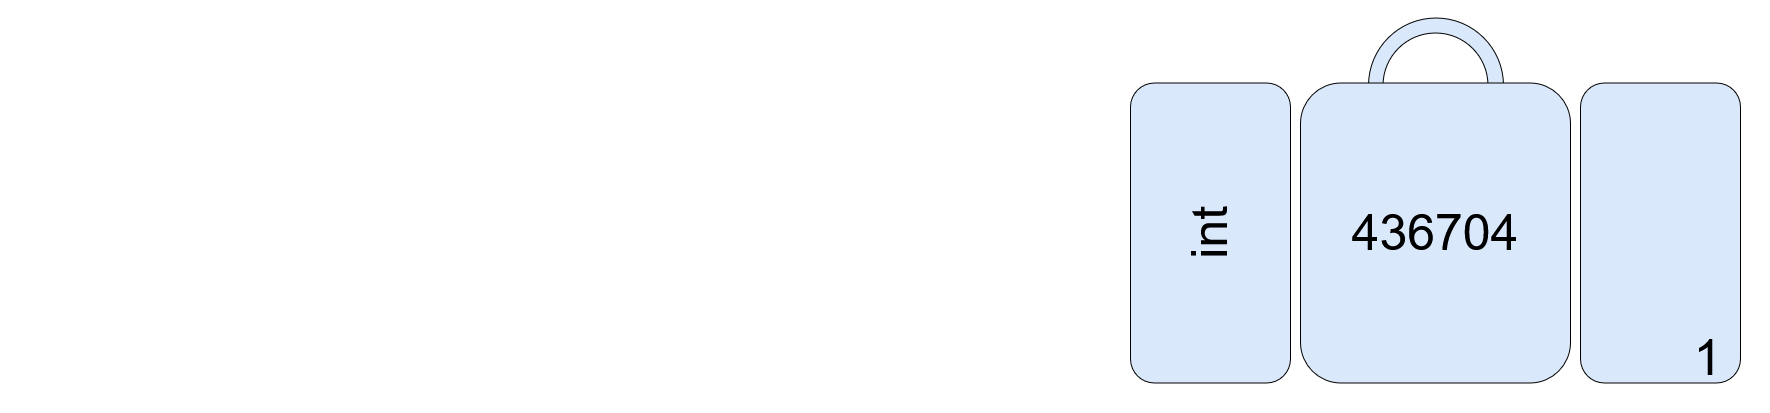
\includegraphics[width=0.8\columnwidth]{../../../FIGURES/python/suitecase/suitecase_0.png}
        \end{figure}
    }

    \only<2>{
        \begin{figure}
            \centering
            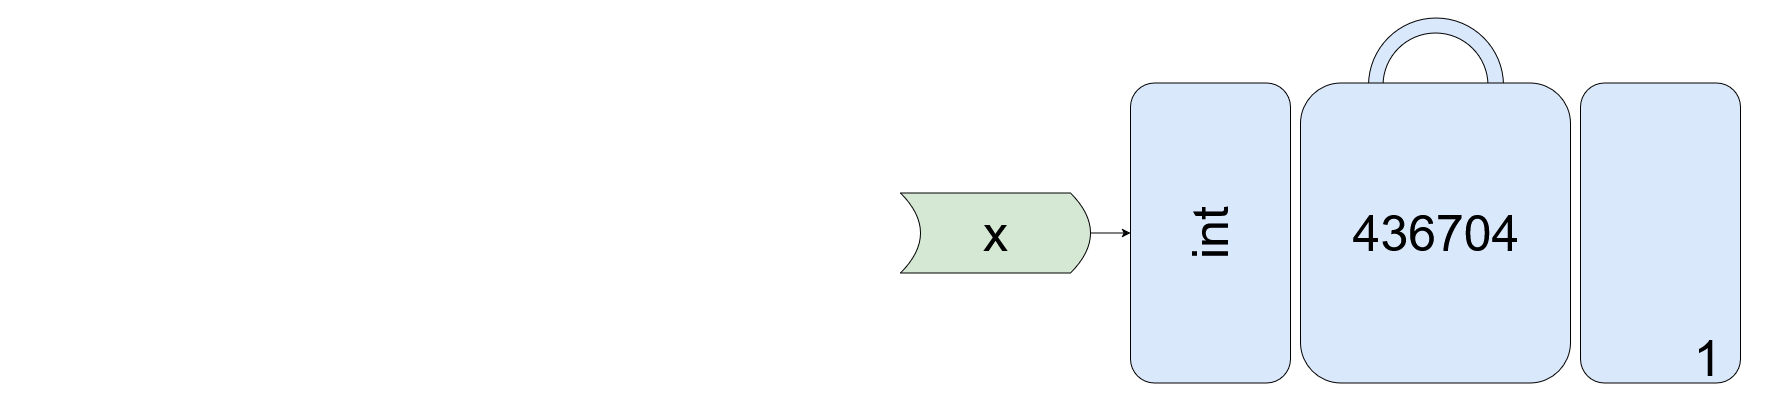
\includegraphics[width=0.8\columnwidth]{../../../FIGURES/python/suitecase/suitecase_1.png}
        \end{figure}
    }

    \only<3>{
        \begin{figure}
            \centering
            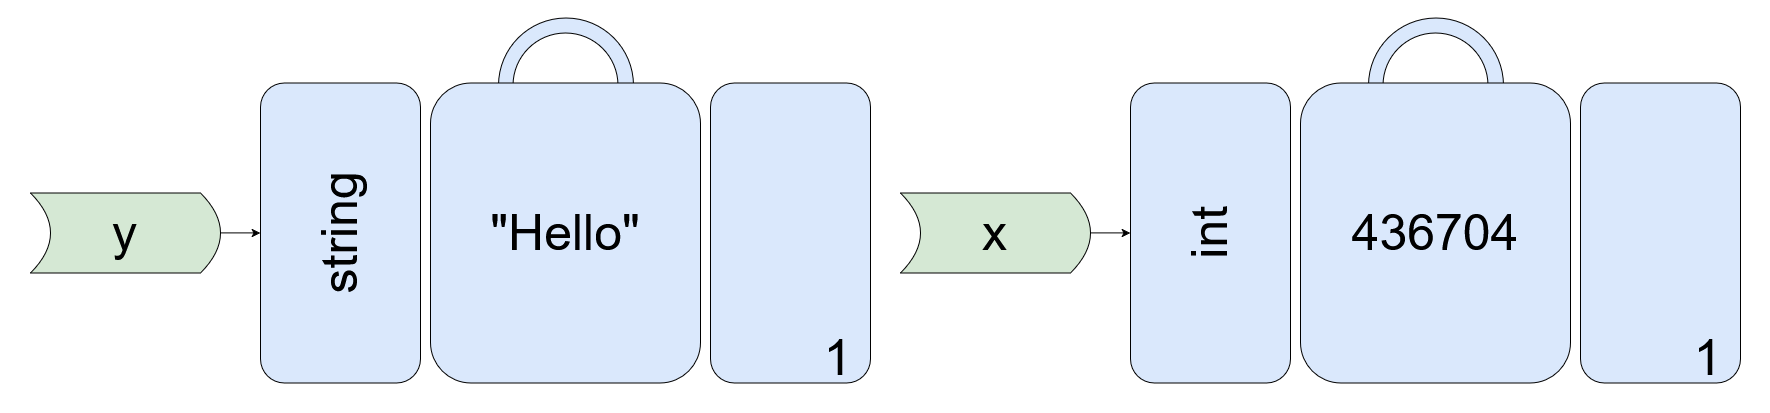
\includegraphics[width=0.8\columnwidth]{../../../FIGURES/python/suitecase/suitecase_2.png}
        \end{figure}
    }

    \only<4->{
        \begin{figure}
            \centering
            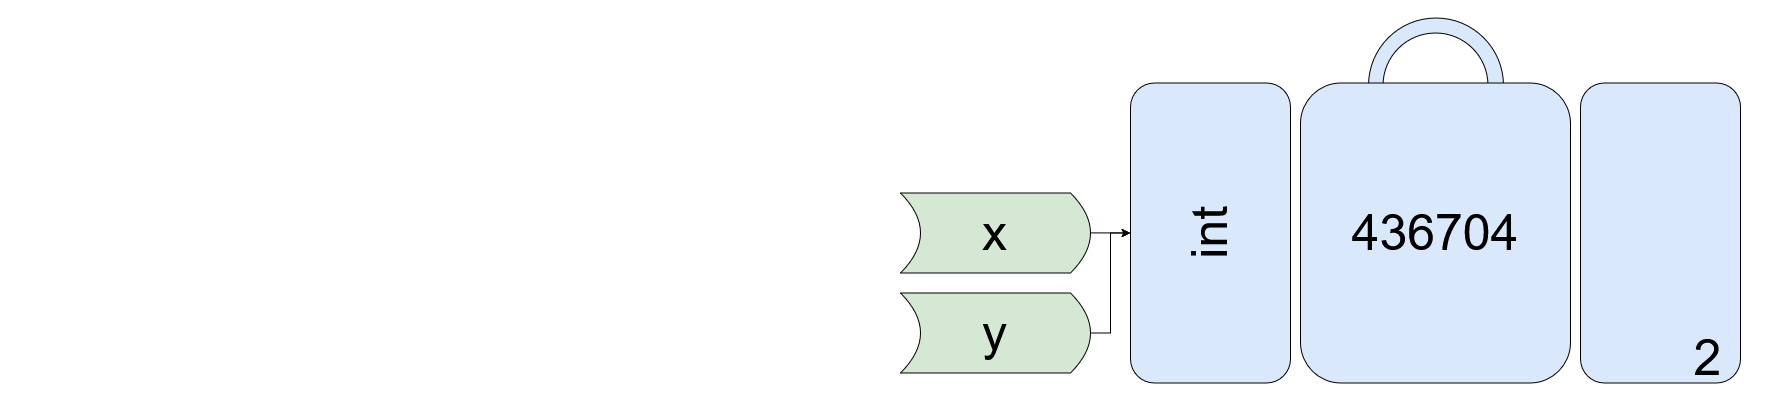
\includegraphics[width=0.8\columnwidth]{../../../FIGURES/python/suitecase/suitecase_3.png}
        \end{figure}
    }

    \begin{block}{Imagine that each Python object is a suitecase}
        \begin{itemize}
            \item Each suitecase store a different value
            \onslide<2->{\item Variables are references to objects (the tags of our suitecases)} 
            \onslide<4->{\item Assigning from a variable (x = y) does not copy an object}
            \onslide<5->{\item Instead, it adds another reference to the same object}
        \end{itemize}
    \end{block}
\end{frame}

\begin{exoframe}{Exercise Time !}
    \begin{block}{Type the following code and note the outputs}
        \begin{CLI}
        x = "hello world" & \\
        y = "hello " & \\
        y += "world" & \\
        & \\
        id(x) & \\ 
        id(y) & \\
        & \\
        x == y & \\ 
        x \tpurple{is} y & \\
        & \\
        4 > 3 \tpurple{is not} True & \\
        \end{CLI}
    \end{block}
    \pause
    \begin{center}
        \Large Why do "==" and "is" produce different outputs ?
    \end{center}
\end{exoframe}

\begin{frame}{is and ==}
    \begin{center}
        \Large
        "is" checks if the suitcases are the same \\
        "==" checks if they have the same stuff inside
    \end{center}
    \pause
    \begin{center}
        \Large
        You will \textit{almost} always want to use "=="
    \end{center}
\end{frame}

\section{}

\begin{frame}
    
\end{frame}

\end{document}
